% =====================================================================
%  sections/sec5.tex —— 5 由六维 A_2 理论得到的 AD 点（原文 pp.22–31）
% =====================================================================
\section{由六维 $A_2$ 理论得到的 AD 点}
\label{sec:a2}

现在我们从六维 $A_2$ 理论出发，把它紧致化在带非正则奇点的黎曼面上，希望在红外得到一个四维 AD 理论。关于黎曼面的类型与非正则奇点数目的分析，与 $\SU(2)$ 情形完全相同，只要盯住 Seiberg--Witten 曲线中的二次微分即可。我们同样只能用黎曼球，并且只能有一个非正则奇点，或一个非正则奇点加一个正则奇点。$A_2$ 理论中非正则奇点的可选类型比 $A_1$ 理论里仅有的两种要多，因此我们立刻得到许多新的 AD 型理论。

\subsection{AD 理论的非正则奇点分类}
\label{sec:5.1}

按照我们对非正则奇点的分类，$\SU(3)$ 群的非正则奇点有如下几种：

\textbf{Type I：}非正则奇点的极点阶与领头阶矩阵为
\begin{equation}
\Phi = z^{r-2}\diag(1,\ \omega,\ \omega^2),\qquad r = n + j/3,\quad 0<j\le 3 .
\label{eq:5.1}\tag{5.1}
\end{equation}
当极点阶为整数时，领头阶矩阵不必具有上述特定形式，其对角元可以取任意三个数；此时还有两个质量参数编码在一阶极点的系数里。若极点阶为分数，则没有质量参数。耦合常数的个数（不含领头阶与一阶极点的系数）由「数出所有与领头阶矩阵相容的形变」得到：
\begin{equation}
\Ncoupling = 2n+j-3\ \ (j\ne 3),\qquad
\Ncoupling = 2(n-1)\ \ (j = 3).
\label{eq:5.2}\tag{5.2}
\end{equation}
这类非正则奇点的牛顿多边形见图 \ref{fig:8}a。

\textbf{Type II：}非正则奇点的极点阶与领头阶矩阵为
\begin{equation}
\Phi = z^{r-2}\diag(0,\ 1,\ \omega),\qquad r = n + 1/2 .
\label{eq:5.3}\tag{5.3}
\end{equation}
一阶极点的系数给出一个质量参数，而耦合常数的个数为
\begin{equation}
\Ncoupling = 2(n-1).
\label{eq:5.4}\tag{5.4}
\end{equation}
这类非正则奇点的牛顿多边形见图 \ref{fig:8}b。

\textbf{Type III：}可以考虑极点阶为整数 $n$ 的非正则奇点的退化。此时非正则奇点由两个整数 $(n_1,n_2)$ 标记，且 $n_1+n_2 = n$，即它含有 $n_1$ 个单杨图与 $n_2$ 个满杨图。质量参数的个数由杨图 $Y_1$ 定：$Y_1$ 是单杨图时有一个，是满杨图时有两个。耦合常数的个数为
\begin{equation}
\Ncoupling = n_1 + 2n_2 - 3 .
\label{eq:5.5}\tag{5.5}
\end{equation}
以上信息汇总在表 \ref{tab:4} 中。

\begin{table}[tbp]
\centering
\caption{由几何数据数参数。这里数的是非正则奇点高阶系数中可能的最大参数个数。}
\label{tab:4}
\begin{tabular}{lcccc}
\toprule
 & 极点阶 & 底空间维数 & 一阶极点 & 高阶极点\\
\midrule
Type I   & $n+j/3$        & $3n+j-7$        & 0 & $2n-3+j$\\
Type I   & $n+1$          & $3n-5$          & 2 & $2(n-1)$＋一个边缘项\\
Type II  & $n+1/2$        & $\frac{3}{2}(n-1)$ & 1 & $2(n-1)$\\
Type III & $n = n_1+n_2$  & $2n_1+n_2-8$    & 2 或 1 & $n_1+2n_2-3$\\
\bottomrule
\end{tabular}
\end{table}

\typo{表 4 的「底空间维数」一栏与正文对不上。按第 \ref{sec:5.1.3} 小节的式 (5.19)，库仑分支维数为 $d = 2n_1+3n_2-8 = 2n+n_2-8$，而表中 Type III 行给的是 $2n_1+n_2-8$；Type II 行给的是 $\frac{3}{2}(n-1)$，对整数 $n$ 并不是整数，按 $\SU(2)$ 情形的同类记账应为 $3n-3$。此处照录原文，未作改动。}

\subsubsection{Type I SCFT：$(A_2,A_{N-1})$ 理论}
\label{sec:5.1.1}

把六维 $A_2$ 理论紧致化在带第一类非正则奇点的黎曼球上，红外就得到一个四维 AD 理论。Seiberg--Witten 曲线可以很容易地用穿刺点上 Higgs 场的形式，从谱曲线求出。实际上，直接从相应非正则奇点的牛顿多边形读出它更方便。牛顿多边形所界定的格点，代表 Seiberg--Witten 曲线中允许出现的单项式。我们用标度不变性把 $z^N$ 项的系数取为一，用平移不变性消去 $z^{N-1}$ 项。$x=2$ 这条线上的点不用，因为 Higgs 场的迹为零。

$(A_2,A_{N-1})$ 理论由 Seiberg--Witten 曲线 $x^3+z^N=0$ 描述，而坐标的标度维数由「要求 Seiberg--Witten 微分 $\lambda = x\,\dd z$ 的维数为一」定出：
\begin{equation}
[x] = \frac{N}{N+3},\qquad [z] = \frac{3}{N+3}.
\label{eq:5.6}\tag{5.6}
\end{equation}
Seiberg--Witten 曲线可以由图 \ref{fig:9} 中牛顿多边形所界定的整数点读出：每个含于其内的点，坐标为 $(m,n)$，对应 Seiberg--Witten 曲线中的一个单项式 $x^mz^n$。

\begin{figure}[tbp]
\centering
% Figure 8 -- a: Newton polygon of the type I irregular singularity
%             b: Newton polygon of the type II irregular singularity
\begin{tikzpicture}[x=1pt,y=1pt,>=stealth,line width=0.5pt]
  \def\u{18.7}
  % ---------------- a) ----------------
  \begin{scope}[shift={(26.2,3.8)}]
    \draw (0,0) -- (0,{6.03*\u});
    \draw (0,0) -- ({4.03*\u},0);
    \foreach \j in {0,...,5} {\fill (0,{\j*\u}) circle[radius=1.9pt];}
    \foreach \i in {1,2,3} {\fill ({\i*\u},0) circle[radius=1.9pt];}
    \draw (0,{5*\u}) -- ({3*\u},0);
  \end{scope}
  \node[inner sep=0pt,font=\fontsize{10.5}{13}\selectfont] at (10.5,110.8) {$a$};
  % ---------------- b) ----------------
  \begin{scope}[shift={(175.7,3.8)}]
    \draw (0,0) -- (0,{6.03*\u});
    \draw (0,0) -- ({6.03*\u},0);
    \foreach \j in {0,...,4} {\fill (0,{\j*\u}) circle[radius=1.9pt];}
    \foreach \i in {1,2,3} {\fill ({\i*\u},0) circle[radius=1.9pt];}
    \fill ({\u},{3*\u}) circle[radius=1.9pt];
    \draw (0,{4*\u}) -- ({\u},{3*\u}) -- ({3*\u},0);
  \end{scope}
  \node[inner sep=0pt,font=\fontsize{10.5}{13}\selectfont] at (150.6,110.8) {$b$};
\end{tikzpicture}

\caption{a：type I 非正则奇点的牛顿多边形。b：type II 非正则奇点的牛顿多边形。}
\label{fig:8}
\end{figure}

一般形变下的 Seiberg--Witten 曲线，用牛顿多边形所界定的格点求出。我们取 $N = 3n-1$ 作详细例子，其他情形类似。Seiberg--Witten 曲线为
\begin{equation}
x^3 + \bigl(v_1z^{2n-1} + \cdots + v_iz^{2n-i} + \cdots + v_{2n}\bigr)x
+ \bigl(z^{3n-1} + u_1z^{3n-3} + \cdots + u_{3n-2}\bigr) = 0 .
\label{eq:5.7}\tag{5.7}
\end{equation}
利用坐标的标度维数，可以求出 Seiberg--Witten 曲线中出现的各种算子的标度维数：
\begin{equation}
[v_i] = \frac{3i-2}{3n+2},\qquad [u_i] = \frac{3+3i}{3n+2}.
\label{eq:5.8}\tag{5.8}
\end{equation}
容易看出：对谱中每一个相关算子 $\sO_i$，都存在另一个耦合常数 $m_i$，使 $D(\sO_i)+D(m_i)=2$。谱中没有质量参数，库仑分支的维数为 $3n-2$；此外还有 $2n$ 个维数小于一的算子，它们是相关形变的耦合常数。

下面把上述数字与非正则奇点定义中的参数作比较。该非正则奇点的极点阶为
\begin{equation}
r = (3n-1)/3 + 2 = (n+1) + 2/3 .
\label{eq:5.9}\tag{5.9}
\end{equation}
由于极点阶是分数，这里没有质量参数，与从 Seiberg--Witten 曲线得到的结果吻合得很好。

来自非正则奇点的耦合常数总数是 $2n+1$ 个。用平移不变性减去一个耦合常数，最终的数字与从 Seiberg--Witten 曲线得到的结果一致。也可以检验：库仑分支的维数与 Hitchin 纤维化底空间的维数相同。

\begin{figure}[tbp]
\centering
% Figure 9 -- lattice points bounded by the Newton polygon, for the three cases a, b, c
\begin{tikzpicture}[x=1pt,y=1pt,>=stealth,line width=0.4pt]
  % ================= a =================
  \begin{scope}[shift={(43.2,152.7)}]
    \def\u{12.75}\def\dd{1.2}\def\oo{2.0}
    \foreach \j in {0,...,6} {\draw (0,{\j*\u}) -- ({7.04*\u},{\j*\u});}
    \foreach \i in {0,...,3} {\draw ({\i*\u},0) -- ({\i*\u},{8.02*\u});}
    \foreach \i/\j in {0/0,1/0,3/0,0/1,1/1,0/2,1/2,0/3,1/3,0/4,0/6}
      {\fill ({\i*\u},{\j*\u}) circle[radius=\dd pt];}
    \foreach \i/\j in {2/0,2/1,0/5} {\draw[fill=white] ({\i*\u},{\j*\u}) circle[radius=\oo pt];}
    \draw[line width=0.8pt] (0,{6*\u}) -- ({3*\u},0);
  \end{scope}
  \node[inner sep=0pt,font=\fontsize{9.6}{12}\selectfont] at (20.4,245.8) {$a$};
  % ================= b =================
  \begin{scope}[shift={(209.0,152.7)}]
    \def\u{12.75}\def\dd{1.2}\def\oo{2.0}
    \foreach \j in {0,...,6} {\draw (0,{\j*\u}) -- ({7.04*\u},{\j*\u});}
    \foreach \i in {0,...,2} {\draw ({\i*\u},0) -- ({\i*\u},{8.02*\u});}
    \foreach \i/\j in {0/0,1/0,3/0,0/1,1/1,0/2,0/3,1/3,0/4,0/5,0/6}
      {\fill ({\i*\u},{\j*\u}) circle[radius=\dd pt];}
    \foreach \i/\j in {2/0,2/1,1/2} {\draw[fill=white] ({\i*\u},{\j*\u}) circle[radius=\oo pt];}
    \draw[line width=0.8pt] (0,{4*\u}) -- ({\u},{3*\u}) -- ({3*\u},0);
  \end{scope}
  \node[inner sep=0pt,font=\fontsize{9.6}{12}\selectfont] at (173.4,245.8) {$b$};
  % ================= c =================
  \begin{scope}[shift={(119.8,50.7)}]
    \def\u{12.7}\def\dd{1.2}\def\oo{2.0}
    \draw (0,0) -- ({6.04*\u},0);
    \foreach \j in {1,2,3,4} {\draw (0,{\j*\u}) -- ({4.04*\u},{\j*\u});}
    \draw (0,0) -- (0,{6.05*\u});
    \draw ({\u},{-3.03*\u}) -- ({\u},{6.05*\u});
    \foreach \i in {2,3} {\draw ({\i*\u},0) -- ({\i*\u},{6.05*\u});}
    \foreach \i/\j in {0/-3,0/-2,1/-2,0/-1,1/-1,0/0,1/0,3/0,0/1,1/1,0/2,1/2,0/3,1/3,0/4}
      {\fill ({\i*\u},{\j*\u}) circle[radius=\dd pt];}
    \foreach \i/\j in {2/-1,2/0,2/1} {\draw[fill=white] ({\i*\u},{\j*\u}) circle[radius=\oo pt];}
    \draw[line width=0.8pt] (0,{-3*\u}) -- ({3*\u},0) -- (0,{4*\u});
  \end{scope}
  \node[inner sep=0pt,font=\fontsize{9.6}{12}\selectfont] at (58.4,105.5) {$c$};
  % the label of the lattice
  \node[inner sep=0pt,font=\fontsize{9.6}{12}\selectfont] at (33.9,194.7) {$N$};
\end{tikzpicture}

\caption{Seiberg--Witten 曲线可以从牛顿多边形所界定的整数点读出。每个含于其内的点，坐标为 $(m,n)$，都对应 Seiberg--Witten 曲线中的一个单项式 $x^mz^n$。}
\label{fig:9}
\end{figure}

应当指出，$(A_2,A_3)$ 理论与 $(A_1,E_6)$ 理论等价，这一点文献 \cite{17} 也讨论过。在 AD 点处，Seiberg--Witten 曲线为
\begin{equation}
x^3 + z^4 = 0 .
\label{eq:5.10}\tag{5.10}
\end{equation}
该理论所有算子的标度维数有公分母 $7$。$(A_2,A_4)$ 理论与 $(A_1,E_8)$ 理论同构，因为不动点处的 Seiberg--Witten 曲线为
\begin{equation}
x^3 + z^5 = 0 ,
\label{eq:5.11}\tag{5.11}
\end{equation}
而标度维数的公分母为 $8$，与文献 \cite{17} 的结论一致。用我们的方法可以构造这两个理论的全部形变；此外，利用非正则奇点中的信息可以直接构造 BPS 箭图，而它们确实具有相应 Dynkin 图的形状 \cite{30}。

\subsubsection{Type II SCFT}
\label{sec:5.1.2}

这一类理论用第二类非正则奇点构造。Seiberg--Witten 曲线同样容易由图 \ref{fig:8}b 的牛顿多边形求出，此时 $N = 2n-1$：
\begin{equation}
x^3 + \bigl(z^{2n-1} + v_1z^{2n-3} + \cdots + v_iz^{2n-2-i} + \cdots + v_{2n-2}\bigr)x
+ \bigl(u_1z^{3n-2} + \cdots + u_iz^{3n-1-i} + \cdots + u_{3n-1}\bigr) = 0 .
\label{eq:5.12}\tag{5.12}
\end{equation}
现在标度维数由奇点 $x^3+z^{2n-1}x=0$ 定出，并要求 Seiberg--Witten 微分 $\lambda = x\,\dd z$ 的维数为一，于是
\begin{equation}
[x] = \frac{2n-1}{2n+1},\qquad [z] = \frac{2}{2n+1}.
\label{eq:5.13}\tag{5.13}
\end{equation}
Seiberg--Witten 曲线中各参数的标度维数也容易求出：
\begin{equation}
[v_i] = \frac{2i+2}{2n+1},\qquad [u_i] = \frac{2i-1}{2n+1}.
\label{eq:5.14}\tag{5.14}
\end{equation}
可以验证：对每个相关算子 $u_i$，都存在一个耦合常数 $m_i$，使 $D(m_i)+D(u_i)=2$。谱中有一个质量参数，与表 \ref{tab:4} 的结论一致。该非正则奇点的极点阶为
\begin{equation}
r = \frac{2n-1}{2} + 2 = (n+1) + \frac{1}{2},
\label{eq:5.15}\tag{5.15}
\end{equation}
因此由表 \ref{tab:4}，非正则奇点中共有 $2n$ 个耦合常数；其中一个可以用平移不变性消去，于是几何给出 $2n-1$ 个参数，与从 Seiberg--Witten 曲线读出的耦合常数个数完全吻合。

\subsubsection{Type III SCFT}
\label{sec:5.1.3}

这一类理论用极点阶为整数 $n$ 的第三类奇点来定义：非正则奇点的前 $n_1$ 个矩阵具有分割 $[2,1]$，后 $n_2$ 个系数具有分割 $[1,1,1]$。Seiberg--Witten 曲线与「领头阶奇点为正则半单」的情形相同，但并非曲线中所有算子都是独立的。

Seiberg--Witten 曲线具有如下形式
\begin{equation}
x^3 + \phi_2(z)x + \phi_3(z) = 0 .
\label{eq:5.16}\tag{5.16}
\end{equation}
我们想算出 $\phi_i(z)$ 中 $z$ 的最高幂次 $d_i$，其系数给出独立的库仑分支算子；这个幂次可以从杨图读出。对单个杨图，它对 $\phi_i(z)$ 的贡献是
\begin{equation}
p_i = i - s_i,
\label{eq:5.17}\tag{5.17}
\end{equation}
其中 $s_i$ 是第 $i$ 个格子的高度。对分割 $[2,1]$，有 $p_2=1$、$p_3=1$；对分割 $[1,1,1]$，极点阶为 $p_2=1$、$p_3=2$。代表独立库仑分支参数的领头项，由下式定出
\begin{equation}
d_i = \sum_j p_i^{(j)} - 2i,
\label{eq:5.18}\tag{5.18}
\end{equation}
求和跑遍非正则奇点定义中出现的所有杨图。于是 $d_2 = n-4$、$d_3 = n_1+2n_2-6$，库仑分支的维数为
\begin{equation}
d = d_2 + d_3 + 2 = 2n_1 + 3n_2 - 8 = 2n + n_2 - 8 .
\label{eq:5.19}\tag{5.19}
\end{equation}

\zhnote{[译者按（无外部依据）：按 (5.17) 的字面读法，$[1,1,1]$（高为三的单列）给出 $s_1=1,s_2=2,s_3=3$，从而 $p_2=p_3=0$，与正文所给 $p_2=1$、$p_3=2$ 不合。正文那组数字恰好是「把 $[1,1,1]$ 当作一行三格」读出的结果（此时三个格子的高度都是 $1$，故 $p_i=i-1$），而也只有这组数字代入 (5.18) 才能得到下文所印的 $d_2=n-4$、$d_3=n_1+2n_2-6$。]}%

AD 点处的 Seiberg--Witten 曲线为 $x^3+z^{3n-6}=0$，$[x]$ 与 $[z]$ 的标度维数为
\begin{equation}
[x] = \frac{n-2}{n-1},\qquad [z] = \frac{1}{n-1},
\label{eq:5.20}\tag{5.20}
\end{equation}
而出现在 $\phi_2$ 与 $\phi_3$ 中的库仑分支算子的最小标度维数为
\begin{equation}
[u_1] = 2[x] - d_2[z] = \frac{n}{n-1},\qquad
[v_1] = 3[x] - d_3[z] = \frac{2n-n_2}{n-1}.
\label{eq:5.21}\tag{5.21}
\end{equation}
于是来自 $\phi_2$ 的相关算子有 $(n-3)$ 个，来自 $\phi_3$ 的相关算子有 $n_2-2$ 个。相关算子的总数为
\begin{equation}
N_{\text{relevant}} = n-3+n_2-2 = n_1+2n_2-5 .
\label{eq:5.22}\tag{5.22}
\end{equation}
非正则奇点定义中的参数个数为 $n_1+2n_2-3$，可见来自非正则奇点的耦合常数是够用的，只是其中有两个被冻结了。

然而，这些理论并不全是 SCFT。原因在于：几何数据里没有严格边缘形变，而库仑分支的谱却可能由标度维数为二的算子构成。我们的解释是，这些理论是渐近自由理论。不含维数为二的算子的理论对应于 $n_2=1$ 或 $n_2=0$，它们给出新的 SCFT。

\subsubsection{Type IV：一个正则奇点加一个非正则奇点}
\label{sec:5.1.4}

我们可以在此前那个只有一个非正则奇点的例子上，再在 $0$ 点加一个正则奇点。就以\allowbreak $(A_1,A_{3n-1})$ 为例，其他情形完全类似。加上一个满正则奇点之后，Seiberg--Witten 曲线为
\begin{equation}
\begin{aligned}
& x^3 + \Bigl(v_1z^{2n-1} + \cdots v_iz^{2n-i} + v_{2n} + \frac{v_{2n+1}}{z} + \frac{v_{2n+2}}{z^2}\Bigr)x\\
& + \Bigl(z^{3n} + \omega z^{3n-2} + u_1z^{3n-2} + \cdots + u_{3n-1} + \frac{u_{3n}}{z} + \frac{u_{3n+1}}{z^2} + \frac{u_{3n+2}}{z^3}\Bigr) = 0 .
\end{aligned}
\label{eq:5.23}\tag{5.23}
\end{equation}
注意这里出现了一个在单奇点情形被禁的新项 $\omega$。另外还有三个库仑分支参数 $v_{2n+1}$、$u_{3n}$、$u_{3n+1}$，其标度维数为
\begin{equation}
[v_{2n+1}] = \frac{6n+3}{3n+3},\qquad
[u_{3n}] = \frac{9n+3}{3n+3},\qquad
[u_{3n+1}] = \frac{9n+6}{n-1}.
\label{eq:5.24}\tag{5.24}
\end{equation}
$v$ 始终是相关算子。$\omega$ 是一个耦合常数，其标度维数为
\begin{equation}
[\omega] = \frac{3}{3n+3}.
\label{eq:5.25}\tag{5.25}
\end{equation}
于是 $\omega$ 与 $v_{2n+1}$ 恰好配对；另外两个参数 $v_{2n+2}$ 与 $u_{3n+2}$ 则只是质量参数，维数分别为 $2$ 与 $3$。

\typo{式 (5.23) 中 $\omega$ 与 $u_1$ 同时乘在 $z^{3n-2}$ 上，同一幂次出现两个系数，这不可能。由 (5.25) 的 $[\omega]=\frac{3}{3n+3}$ 反推：若 $\omega$ 乘的是 $z^{3n-1}$，则 $[\omega]+(3n-1)[z]=3[x]$ 恰好成立；而 $z^{3n-1}$ 正是单奇点情形被平移不变性消去、加了一个穿刺点之后重新出现的那一项（与 (4.7) 的 $u_1z^{N-1}$ 完全平行）。故原文 $z^{3n-2}$ 应为 $z^{3n-1}$。又 (5.24) 中 $[u_{3n+1}]$ 的分母印作 $n-1$；由单项式 $u_{3n+1}z^{-2}$ 的维数等于 $3[x]$ 反算，分母应为 $3n+3$。两处均照录原文。}

\typo{第 \ref{sec:5.1.4} 小节开头原文写作「就以 $(A_1,A_{3n-1})$ 为例」。本节处理的是六维 $A_2$ 理论，且式 (5.23) 的曲线与 $(A_2,A_{3n-1})$ 相符，故此处下标 $1$ 应为 $2$。译文照录原文。}

若正则奇点是单的，则只有 $v_{2n+1}$ 与 $u_{3n}$ 是独立的库仑分支算子，且只有一个新质量参数。

\subsection{三维镜像理论}
\label{sec:5.2}

若把四维理论紧致化在一个圆上并流向深红外，红外理论是一个三维 $\sN{=}4$ SCFT $A$。只要极点阶是整数，就可以直接从非正则奇点求出它的镜像理论 $B$ \cite{44}。设前 $n_1$ 个分割的杨图为 $[2,1]$，后 $n_2$ 个分割的杨图为 $[1,1,1]$，则可以按图 \ref{fig:10} 配上一个箭图。若 $n_2=0$，则只有两个节点，其秩分别为 $1$ 与 $2$，两节点之间有 $n-2$ 支箭；此时原理论的质量参数个数为一。

有几个容易做的检验：该箭图的希格斯分支维数为 $2n+n_2-8$，恰好是原理论的库仑分支；FI 参数的个数正好是箭图节点数减一，与原理论的质量参数个数相符。正则奇点的箭图支链已在 \cite{38} 中给出，它完全由杨图确定，见图 \ref{fig:10}。要把正则奇点的箭图支链粘到非正则奇点的箭图上，需要按非正则奇点箭图的模式把正则奇点的 $U(3)$ 味对称性劈开，即：若非正则奇点的箭图有三个 $U(1)$ 节点，就把正则奇点的 $U(3)$ 味对称性劈成三个 $U(1)$。粘合通过把这些 $U(1)$ 味对称性与非正则奇点箭图的 $U(1)$ 规范群认同来实现。

\begin{figure}[tbp]
\centering
% Figure 10 -- a) U(1)xU(1) with n-2 bifundamentals; b) the regular puncture legs;
%              c) U(2) split into two U(1); d) after gluing
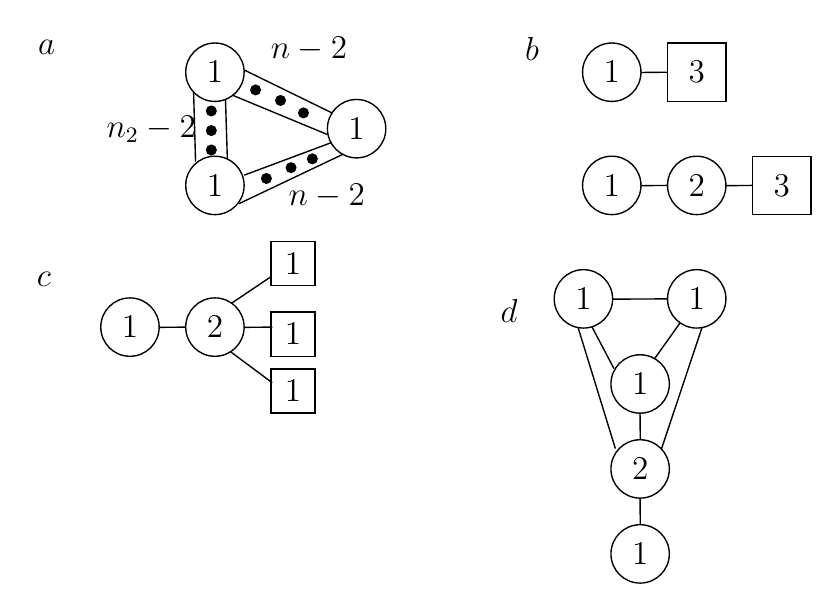
\begin{tikzpicture}[x=1pt,y=1pt,>=stealth,line width=0.5pt,
    nd/.style={circle,draw,fill=white,inner sep=0pt,minimum size=21.1pt,
               font=\fontsize{11.5}{14}\selectfont},
    sq/.style={rectangle,draw,fill=white,inner sep=0pt,minimum width=21.2pt,
               minimum height=21.1pt,font=\fontsize{11.5}{14}\selectfont},
    rr/.style={font=\fontsize{11.5}{14}\selectfont}]
  % =================== a) ===================
  % ribbon between the two left nodes (vertical)
  \draw (65.2,188.5) -- (65.9,163.5);
  \draw (76.7,186.6) -- (77.4,164.1);
  % ribbon to the right node, upper
  \draw (79.0,187.6) -- (113.5,173.3);
  \draw (83.5,196.6) -- (115.4,181.0);
  % ribbon to the right node, lower
  \draw (81.6,148.3) -- (119.9,166.5);
  \draw (83.5,158.6) -- (114.8,170.3);
  \foreach \x/\y in {91.5/157.4, 100.4/161.3, 108.1/164.5,
                     71.6/167.7, 71.6/174.7, 71.6/181.8,
                     104.9/181.1, 96.6/185.6, 87.6/189.4}
    {\fill (\x,\y) circle[radius=2.0pt];}
  \node[nd] at (72.9,195.8) {1};
  \node[nd] at (72.9,154.9) {1};
  \node[nd] at (124.1,175.4) {1};
  \node[rr] at (106.9,204.2) {$n-2$};
  \node[rr] at (113.3,151.1) {$n-2$};
  \node[rr] at (49.9,175.2) {$n_2-2$};
  \node[rr] at (12.1,204.8) {$a$};
  \node[rr] at (187.5,204.2) {$b$};
  % =================== b) ===================
  \draw (226.2,195.7) -- (237.1,195.8);
  \node[nd] at (216.3,195.8) {1};
  \node[sq] at (247.0,195.85) {3};
  \draw (226.2,154.8) -- (237.1,154.9);
  \draw (256.9,154.8) -- (267.8,154.9);
  \node[nd] at (216.3,154.9) {1};
  \node[nd] at (247.0,154.9) {2};
  \node[sq] at (277.75,154.85) {3};
  % =================== c) ===================
  \draw (52.1,103.6) -- (63.0,103.7);
  \draw (82.8,103.6) -- (93.7,103.7);
  \draw (78.4,94.9) -- (93.6,83.6);
  \draw (79.0,112.4) -- (93.0,121.8);
  \draw (93.1,118.7) rectangle (109.1,134.7);
  \draw (93.1,93.1) rectangle (109.1,109.1);
  \draw (93.1,72.6) rectangle (109.1,88.6);
  \node[nd] at (42.2,103.7) {1};
  \node[nd] at (72.9,103.7) {2};
  \node[rr] at (101.1,126.7) {1};
  \node[rr] at (101.1,101.1) {1};
  \node[rr] at (101.1,80.6) {1};
  \node[rr] at (11.1,121.0) {$c$};
  % =================== d) ===================
  \draw (216.0,113.8) -- (237.1,113.9);
  \draw (208.4,105.2) -- (217.1,88.7);
  \draw (231.5,91.9) -- (241.4,105.8);
  \draw (203.4,105.9) -- (217.6,59.8);
  \draw (234.1,59.2) -- (249.7,105.9);
  \draw (226.5,73.9) -- (226.6,63.0);
  \draw (226.5,43.8) -- (226.6,32.3);
  \node[nd] at (206.05,113.9) {1};
  \node[nd] at (247.0,113.9) {1};
  \node[nd] at (226.55,83.15) {1};
  \node[nd] at (226.55,52.45) {2};
  \node[nd] at (226.55,21.75) {1};
  \node[rr] at (179.2,109.5) {$d$};
\end{tikzpicture}

\caption{a：带 $n_1$ 个单杨图与 $n_2$ 个满杨图、极点阶为 $n=n_1+n_2$ 的非正则奇点所对应的箭图。b：单正则穿刺点与满正则穿刺点所对应的箭图支链。c：把正则奇点箭图支链的 $U(3)$ 味对称性劈成三个 $U(1)$ 因子。d：把劈开后的正则奇点箭图支链粘到非正则奇点上，构成三维镜像理论；这里有一个阶为 $3$、领头阶为正则半单的非正则奇点，还有一个满正则奇点。}
\label{fig:10}
\end{figure}

\subsection{中心荷 $a$ 与 $c$}
\label{sec:5.3}

求中心荷 $a$ 与 $c$ 的策略与我们在 $\SU(2)$ 理论中做的完全一样：先用三维镜像对称算出中心荷，再用结果找出这一类理论的普适函数 $R(B)$；最后用 $R(B)$ 算出这一类中其他理论的中心荷。

我们先考虑 $N=3n$ 的 $(A_2,A_{N-1})$ 理论，因为它的三维镜像理论是已知的。用牛顿多边形写出的 Seiberg--Witten 曲线具有如下形式：
\begin{equation}
x^3 + \bigl(v_1z^{2n-1} + \cdots v_iz^{2n-i} + v_{2n}\bigr)x
+ \bigl(z^{3n} + u_1z^{3n-2} + \cdots + u_{3n-1}\bigr) = 0 .
\label{eq:5.26}\tag{5.26}
\end{equation}
$x$ 与 $z$ 的标度维数为
\begin{equation}
[x] = \frac{3n}{3n+3},\qquad [z] = \frac{3}{3n+3}.
\label{eq:5.27}\tag{5.27}
\end{equation}
用这些信息可以求出各算子的标度维数：
\begin{equation}
[v_i] = \frac{3i}{3n+3},\qquad [u_i] = \frac{3i+3}{3n+3}.
\label{eq:5.28}\tag{5.28}
\end{equation}
镜像理论的库仑分支维数为二，因此原理论的有效希格斯分支维数也是二。利用公式
\begin{equation}
2a-c = \frac{1}{4}\sum_{i=1}^{r}\bigl(2D(u_i)-1\bigr),\qquad
a-c = -\frac{1}{12},
\label{eq:5.29}\tag{5.29}
\end{equation}
即得中心荷
\begin{equation}
a = \frac{1}{4}\sum_{i=1}^{r}\bigl(2D(u_i)-1\bigr) + \frac{1}{12}
= \frac{-5-5n+24n^2}{12(1+n)},\qquad
c = \frac{1}{4}\sum_{i=1}^{r}\bigl(2D(u_i)-1\bigr) + \frac{1}{6}
= \frac{-1+n-6n^2}{3+3n}.
\label{eq:5.30}\tag{5.30}
\end{equation}
注意求和只跑遍所有维数大于一的算子。

现在用上面的结果和公式 (2.8) 来算 $R(B)$。$R(A)$ 容易由谱的标度维数求出：
\begin{equation}
R(A) = \sum_{i=n+2}^{2n}\Bigl[\frac{3i}{3n+3}-1\Bigr]
+ \sum_{i=n+1}^{3n-1}\Bigl[\frac{3i+3}{3n+3}-1\Bigr]
= \frac{n(-3+5n)}{2(1+n)} .
\label{eq:5.31}\tag{5.31}
\end{equation}
把上面得到的中心荷代入公式 (2.8)，得到
\begin{equation}
R(B) = \frac{3N(N-1)}{2(N+3)} .
\label{eq:5.32}\tag{5.32}
\end{equation}
我们假定 $R(B)$ 具有普适形式、可以用于这一类中的其他理论，于是它们的中心荷就容易算了。类似地，只要三维镜像理论是显式已知的，就能求出其他 SCFT 的中心荷，这包括 type III SCFT 与 type IV SCFT——它们的非正则奇点都有三维镜像箭图。这部分留给感兴趣的读者。

\subsection{由 $\SU(3)$ QCD 得到的 AD 理论}
\label{sec:5.4}

现在我们用奇点碰撞的想法来找出 $\SU(3)$ QCD 可能的 AD 轨迹。给定 $N_f$ 的理论，其非正则奇点的类型并不唯一，而依赖于 $N_f = n_1+n_2$（$n_i\le 3$）的一个分割 \cite{32}；这是因为可以在左右两侧放不同数目的膜 \cite{45}。奇点类型按 $n$ 的取值分为：
\begin{enumerate}[label=\textup{\alph*.}]
  \item $n=0$，$\Phi = \lambda z^{-1-1/3}\diag(1,\omega,\omega^2)+\cdots$。这是 type I 非正则奇点。
  \item $n=1$，$\Phi = \lambda z^{-1-1/2}\diag(0,1,\omega)+\cdots$。这是 type II 非正则奇点。
  \item $n=2$，$\Phi = \lambda z^{-2}\diag(-2,1,1) + z^{-1}(m_1,m_2,m_3)+\cdots$。这是 type III 非正则奇点。
  \item $n=3$，此时有一个满正则奇点与一个单正则奇点。
\end{enumerate}

碰撞规则可以由「合成后的非正则奇点所编码的参数个数与原奇点相同」这一要求定出。规则如下：
\begin{enumerate}
  \item 在分数极点情形，只能让两个同类型的非正则奇点相撞，或让分数阶的非正则奇点与「领头阶矩阵为正则半单」的整数阶非正则奇点相撞。
  \item 也可以让分数阶的非正则奇点与满正则奇点相撞。
  \item 两个非正则奇点相撞，要求它们是仅剩的奇点；非正则奇点与正则奇点相撞，要求至少有三个奇点。
\end{enumerate}
在所有情形下，合成后奇点的极点阶就是原来两者的极点阶之和。下面用这些规则玩一玩。

对 $N_f=0$，有两个完全相同的、极点阶为 $1+1/3$ 的 type I 非正则奇点；它们相撞后产生一个极点阶为 $r = 2+2/3$ 的 type I 非正则奇点。由这个非正则奇点得到的 AD 理论是 $(A_2,A_1)$ 理论。文献 \cite{12} 中找到的 AD 理论实际上是 $(A_1,A_2)$ 理论，而我们后面会说明这两者确实相同。UV 中有两个参数，它们正是库仑分支算子；相应的 AD 理论也有两个算子：一个相关算子与一个耦合常数。于是 UV 参数与 IR 参数相匹配。

对 $N_f=2$，若在左右两侧各放一个膜，则有两个 type II 非正则奇点。它们相撞后产生一个 $r=3$ 的 type I 奇点。与这个奇点对应的 AD 点，实际上就是文献 \cite{12} 中找到的那个，也就是 $(A_2,A_2)$ 理论。UV 理论有四个参数：两个质量参数与两个库仑分支算子。这个 AD 理论也有两个质量参数、一个库仑分支算子与一个耦合常数。

对 $N_f=3$，把三个膜都放在一侧，则有一个 type I 非正则奇点、一个满正则奇点与一个单正则奇点。非正则奇点与满正则奇点相撞，产生一个 $r=2+1/3$ 的 type I 非正则奇点。于是我们的 AD 理论由一个极点阶为 $r=2+1/3$ 的 type I 非正则奇点与一个单正则奇点描述。这个 AD 理论是 type IV 理论，有五个参数，与 UV 理论相匹配。

对 $N_f=4$，分割为 $4 = 3+1$。此时有一个 type II 非正则奇点、一个满正则奇点与一个单正则奇点。把非正则奇点与满正则奇点相撞，就得到一个有六个参数的 type IV AD 理论。

至于 $N_f=5$ 的理论，我们无法通过碰撞非正则奇点找到任何 AD 理论。

\subsection{type IV SCFT 的用处}
\label{sec:5.5}

当球上有不止一个非正则奇点时，四维理论是渐近自由理论。在「退化」极限中出现的新物质内容，是由两孔球表示的 type IV SCFT。例如，若有两个非正则奇点，则四维理论是一个 $\SU(3)$ 规范群与两个 type IV SCFT 耦合，而这两个 SCFT 分别由相应的满正则奇点与相应的非正则奇点定义。物理图像与图 \ref{fig:6} 所画相同。

有了上述观察，对于亏格 $g$ 的黎曼面上任意组合的非正则奇点与正则奇点，写出相应四维理论的物质内容与弱耦合规范群（包括渐近自由的规范群）都不成问题。\footnote{原文在此写作 "asymptotical gauge group"，按上下文应指渐近自由（asymptotically free）的规范群。}几何上，所有非正则奇点都应当位于黎曼面的边界上，而正则奇点则坐在体内。例子见图 \ref{fig:11}：每条边界代表一个非正则奇点，物理上它代表一个与体内耦合的 type IV AD 理论。

\begin{figure}[tbp]
\centering
% Figure 11 -- Riemann surface with regular and irregular punctures
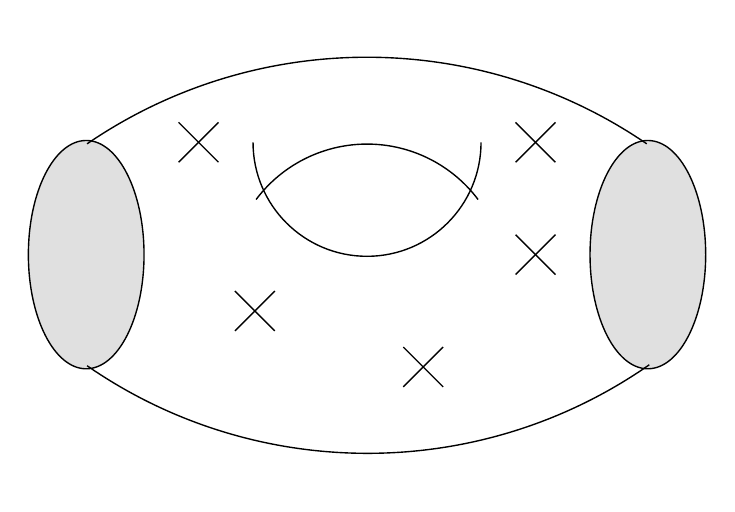
\begin{tikzpicture}[x=1pt,y=1pt,scale=1.10,transform shape,>=stealth,line width=0.5pt]
  \def\cr#1#2{\draw (#1-6.55,#2-6.55) -- (#1+6.55,#2+6.55);
               \draw (#1-6.55,#2+6.55) -- (#1+6.55,#2-6.55);}
  % ---- the two ends of the surface ----
  \draw[fill=black!12] (25.1,85.5) ellipse[x radius=19pt,y radius=37.5pt];
  \draw[fill=black!12] (209.6,85.5) ellipse[x radius=19pt,y radius=37.5pt];
  % ---- upper and lower boundary ----
  \draw (25.4,121.9) arc[start angle=124.4,end angle=55.6,radius=162.7pt];
  \draw (25.4,49.0) arc[start angle=235.3,end angle=304.9,radius=161.8pt];
  % ---- the cycle drawn on the surface ----
  \draw (80.9,103.6) arc[start angle=143.1,end angle=36.9,radius=45.6pt];
  \draw (79.9,122.4) arc[start angle=180,end angle=360,radius=37.45pt];
  % ---- punctures ----
  \cr{62.0}{122.4}
  \cr{172.7}{122.4}
  \cr{172.7}{85.5}
  \cr{80.5}{67.0}
  \cr{135.8}{48.6}
\end{tikzpicture}

\caption{带有一串正则奇点与非正则奇点的黎曼面；相应的四维理论是一个渐近自由理论，它由把 type IV Argyres--Douglas 理论与三孔球构成的 SCFT 规范化得到。}
\label{fig:11}
\end{figure}
